\secnumbersection{VALIDACIÓN DE LA SOLUCIÓN}

La validación de la solución propuesta constituye una etapa crítica que permite demostrar la efectividad de los dos bloques desarrollados en diferentes entornos y condiciones. Esta validación se estructura en dos componentes principales: la validación del bloque de bajas frecuencias (DRAFTS++) y la validación del bloque de altas frecuencias (High Frequency Detection).

\subsection{VALIDACIÓN DEL BLOQUE DE BAJAS FRECUENCIAS (DRAFTS++)}

La validación de DRAFTS++ se realizó mediante un proceso incremental que permitió verificar cada componente del sistema antes de su implementación completa. Este enfoque metodológico aseguró la robustez y confiabilidad del pipeline desarrollado.

\subsubsection{Validación Inicial con Dataset de Entrenamiento}

El proceso de validación inició con el dataset FAST-FREX (FAST dataset for Fast Radio bursts EXploration), el mismo conjunto de datos utilizado para el entrenamiento de los modelos de detección. Esta etapa fue fundamental para validar todas las nuevas funcionalidades implementadas en DRAFTS++, incluyendo los nuevos tipos de visualización y el manejo de archivos de entrada, antes incluso del desarrollo del sistema de chunking.

\begin{figure}[H]
    \centering
    \includegraphics[width=\textwidth]{figures/FRB20180301_0001_slice003.png}
    \caption{Detección de un Fast Radio Burst (FRB) del dataset de entrenamiento FAST-FREX. El panel superior muestra el mapa de dispersión (DM vs. Tiempo) con el evento resaltado. Los paneles inferiores presentan el SNR en cascada crudo, el SNR dedispersado y el SNR del parche candidato, confirmando una detección robusta con un SNR de 5.9$\sigma$.}
    \label{fig:frb20180301_0001_slice003}
\end{figure}

\begin{figure}[H]
    \centering
    \includegraphics[width=\textwidth]{figures/FRB20201124_0009_slice004.png}
    \caption{Detección de un segundo Fast Radio Burst (FRB) del dataset de entrenamiento FAST-FREX. Se observa una detección robusta con SNR de 16.5$\sigma$ después de la dedispersión, confirmando la efectividad del sistema en el dataset de entrenamiento.}
    \label{fig:frb20201124_0009_slice004}
\end{figure}

\subsubsection{Validación de Continuidad Temporal y Time Domain}

Una vez establecida la funcionalidad básica, se procedió a evaluar una característica crítica para cualquier pipeline de detección: la continuidad temporal y la precisión en el dominio del tiempo. Para esta validación se utilizó el pulsar de prueba B0355+54\_FB\_20220918, seleccionado por sus características ideales para este propósito:

\begin{itemize}
    \item \textbf{Brightness}: Pulsar sumamente brillante que facilita la detección
    \item \textbf{Periodo de rotación}: 0.156 segundos
    \item \textbf{Duración del archivo}: 117.23 segundos (1 minuto 57 segundos)
    \item \textbf{Pulsos esperados}: 752 pulsos teóricos
\end{itemize}

Los resultados obtenidos fueron altamente satisfactorios:
\begin{itemize}
    \item \textbf{Pulsos detectados}: 732 de 752 esperados (97.3\% de eficiencia)
    \item \textbf{Clasificación}: 718 clasificados como BURSTS, 14 como NO BURSTS
\end{itemize}

\begin{figure}[H]
    \centering
    \includegraphics[width=\textwidth]{figures/B0355+54_FB_20220918_slice000.png}
    \caption{Validación de continuidad temporal - Slice 000: Se observan 7 pulsos detectados en el primer segundo de observación, demostrando la capacidad del sistema para detectar eventos periódicos con alta precisión temporal. Todos los pulsos fueron clasificados como BURSTS con scores de clasificación superiores a 0.99.}
    \label{fig:b0355_slice000}
\end{figure}


\begin{figure}[H]
    \centering
    \includegraphics[width=\textwidth]{figures/B0355+54_FB_20220918_slice001.png}
    \caption{Validación de continuidad temporal - Slice 001: Continuidad perfecta en el segundo slice, mostrando 5 pulsos clasificados como BURSTS y 1 como NO BURST. La consistencia en la detección temporal confirma la robustez del sistema de procesamiento por ventanas.}
    \label{fig:b0355_slice001}
\end{figure}

Este resultado confirmó la capacidad del sistema para mantener la continuidad temporal entre ventanas de procesamiento y validó la precisión de las redes de detección pre-entrenadas de DRAFTS en condiciones controladas.

\begin{figure}[H]
    \centering
    \includegraphics[width=\textwidth]{figures/B0355+54_FB_20220918_slice013.png}
    \caption{Caso de estudio: Pulso dudoso en la clasificación. El evento \#6 (DM: 55.5, Time: 13.93s) muestra un score de detección alto (0.73) pero un score de clasificación bajo (0.27), resultando en clasificación "NO BURST". El evento \#4 (DM: 54.6, Time: 14.08s) presenta un score de detección muy alto (0.81) pero clasificación muy baja (0.09). Esto demuestra la capacidad del sistema para detectar señales ambiguas que requieren revisión manual.}
    \label{fig:b0355_slice013}
\end{figure}

\subsubsection{Validación con Datos del FRB 121102}

Para evaluar el rendimiento del sistema en condiciones reales y con archivos de gran tamaño, se utilizó el dataset del FRB 121102, basado en el trabajo de \cite{cruces2020frb121102}. Este dataset presentó desafíos computacionales significativos que requirieron la implementación del sistema de chunking y la optimización del consumo de recursos.

\paragraph{Metodología de Validación}

La validación se realizó mediante una comparación directa con los resultados reportados en la literatura por Cruces et al. (2020) \cite{cruces2020frb121102}, quienes estudiaron el comportamiento repetitivo de FRB 121102 incluyendo periodicidad, tiempos de espera y distribución de energía. Se analizaron los mismos archivos de observación para asegurar una evaluación equitativa.

\paragraph{Resultados de Detección del Pipeline DRAFTS++}

El análisis de FRB121102 con el pipeline DRAFTS++ produjo 41 detecciones distribuidas en 6 archivos de observación (3096, 3098, 3099, 3100, 3101, 3102). Los resultados se clasificaron en tres categorías principales:

\begin{enumerate}
    \item \textbf{Bursts confirmados por literatura} (24 eventos): Detectados tanto por DRAFTS++ como reportados por Cruces et al. (2020)
    \item \textbf{Nuevos candidatos sin confirmar} (15 eventos): Detectados únicamente por DRAFTS++, pendientes de validación científica
    \item \textbf{Nuevos eventos confirmados} (2 eventos): Detectados por DRAFTS++ y 100\% confirmados por el grupo de astrónomos colaboradores
\end{enumerate}

\subparagraph{Bursts Confirmados por Literatura}

La Tabla \ref{tab:confirmed_bursts} presenta los 24 bursts que fueron detectados tanto por el pipeline DRAFTS++ como reportados en la literatura por Cruces et al. (2020), demostrando la capacidad del sistema para identificar correctamente eventos conocidos.

\begin{table}[H]
    \centering
    \caption{Bursts de FRB121102 confirmados por literatura (detectados por DRAFTS++ y reportados por Cruces et al. 2020). \textit{Fuente: Elaboración propia basada en Cruces et al. (2020) \cite{cruces2020frb121102}.}}
    \label{tab:confirmed_bursts}
    \begin{tabular}{|c|c|c|c|}
        \hline
        \textbf{File} & \textbf{DM} & \textbf{Time(s)} & \textbf{MJD} \\
        \hline
        3096 & 564.15 & 114.059783 & 58440.83884126 \\
        3096 & 564.64 & 2172.299182 & 58440.86266456 \\
        3098 & 564.77 & 229.680524 & 58440.92373659 \\
        3098 & 565.35 & 1359.279991 & 58440.93681124 \\
        3098 & 563.5 & 3445.629 & 58440.96095990 \\
        3099 & 557.55 & 2331.324798 & 58440.98983520 \\
        3099 & 564.17 & 3111.182227 & 58440.99886157 \\
        3100 & 565.38 & 254.527406 & 58441.00759278 \\
        3100 & 557.11 & 310.032903 & 58441.00823545 \\
        3100 & 563.91 & 686.839999 & 58441.01259666 \\
        3100 & 564.75 & 942.375786 & 58441.01555436 \\
        3100 & 563.87 & 1148.701027 & 58441.01794252 \\
        3100 & 565.97 & 1253.032154 & 58441.01915005 \\
        3100 & 564.96 & 2090.123919 & 58441.02883908 \\
        3100 & 557.7 & 2090.126104 & 58441.02883929 \\
        3100 & 563.53 & 2172.314365 & 58441.02979044 \\
        3101 & 558.49 & 1160.627268 & 58441.05983026 \\
        3101 & 557.92 & 1174.354439 & 58441.05998916 \\
        3101 & 558.01 & 1297.028219 & 58441.06140906 \\
        3101 & 566.12 & 1571.448422 & 58441.06458515 \\
        3101 & 565.31 & 1814.433191 & 58441.06739762 \\
        3102 & 563.14 & 1571.362789 & 58441.10636851 \\
        3102 & 556.67 & 1823.937659 & 58441.10929213 \\
        3102 & 563.94 & 2099.014533 & 58441.11247584 \\
        \hline
    \end{tabular}
\end{table}

\subparagraph{Nuevos Candidatos Sin Confirmar}

La Tabla \ref{tab:candidate_bursts} presenta los 15 nuevos candidatos detectados únicamente por DRAFTS++ que aún requieren confirmación científica. Estos representan el potencial de descubrimiento del sistema.

\begin{table}[H]
    \centering
    \caption{Nuevos candidatos a bursts detectados únicamente por DRAFTS++ (pendientes de confirmación científica). \textit{Fuente: Elaboración propia}.}
    \label{tab:candidate_bursts}
    \begin{tabular}{|c|c|c|c|}
        \hline
        \textbf{File} & \textbf{DM} & \textbf{Time(s)} & \textbf{MJD} \\
        \hline
        3096 & 579.6 & 1208.742 & 58440.851511757 \\
        3096 & 565.46 & 2789.205716 & 58440.86980499 \\
        3096 & 484.19 & 3475.569268 & 58440.87775151 \\
        3098 & 581.24 & 2745.689702 & 58440.93681364 \\
        3098 & 571.6 & 3179.596 & 58440.95285796 \\
        3099 & 411.4 & 480.104 & 58440.96840787 \\
        3099 & 420.31 & 2491.019865 & 58440.99168722 \\
        3099 & 396.29 & 3205.235999 & 58440.99995461 \\
        3100 & 404.21 & 2638.652812 & 58441.03519230 \\
        3100 & 260.22 & 3037.433692 & 58441.03980380 \\
        3101 & 380.95 & 841.313157 & 58441.05613900 \\
        3101 & 555.9 & 2973.492401 & 58441.08081351 \\
        3102 & 564.79 & 841.23932 & 58441.09791759 \\
        3102 & 565.27 & 3179.698804 & 58441.12498428 \\
        \hline
    \end{tabular}
\end{table}

\subparagraph{Nuevos Eventos Confirmados}

La Tabla \ref{tab:new_confirmed_bursts} presenta los 2 nuevos eventos de bursts que fueron detectados por DRAFTS++ y posteriormente 100\% confirmados por el grupo de astrónomos colaboradores.

\begin{table}[H]
    \centering
    \caption{Nuevos eventos de bursts 100\% confirmados por el grupo de astrónomos colaboradores. \textit{Fuente: Elaboración propia}.}
    \label{tab:new_confirmed_bursts}
    \begin{tabular}{|c|c|c|c|}
        \hline
        \textbf{File} & \textbf{DM} & \textbf{Time(s)} & \textbf{MJD} \\
        \hline
        3096 & 563.6 & 2421.559296 & 58440.86554968 \\
        3102 & 564.88 & 723.455399 & 58441.09655428 \\
        \hline
    \end{tabular}
\end{table}

Estos dos nuevos eventos representan descubrimientos científicos genuinos realizados por DRAFTS++, como se muestra en las Figuras \ref{fig:new_event_3096} y \ref{fig:new_event_3102}. Las visualizaciones confirman la detección robusta de ambos eventos con altos valores de SNR después de la dedispersión.

\begin{figure}[H]
    \centering
    \includegraphics[width=\textwidth]{figures/3096_0001_00_8bit_slice039.png}
    \caption{Primer nuevo evento confirmado de FRB121102 detectado por DRAFTS++ en el archivo 3096\_0001\_00\_8bit, slice 039. El evento muestra DM=563.6 pc cm$^{-3}$ y Time=2421.559296s, con un SNR de 6.3$\sigma$ después de la dedispersión. La detección fue 100\% confirmada por el grupo de astrónomos colaboradores. \textit{Fuente: Elaboración propia}.}
    \label{fig:new_event_3096}
\end{figure}

\begin{figure}[H]
    \centering
    \includegraphics[width=\textwidth]{figures/3102_0001_00_8bit_slice040.png}
    \caption{Segundo nuevo evento confirmado de FRB121102 detectado por DRAFTS++ en el archivo 3102\_0001\_00\_8bit, slice 040. El evento muestra DM=564.88 pc cm$^{-3}$ y Time=723.455399s, con un SNR de 12.0$\sigma$ después de la dedispersión. Este evento representa uno de los bursts más brillantes detectados en el dataset y fue 100\% confirmado por el grupo de astrónomos colaboradores. \textit{Fuente: Elaboración propia}.}
    \label{fig:new_event_3102}
\end{figure}

\paragraph{Análisis de Distribución Temporal}

Para visualizar la distribución temporal de los diferentes tipos de detecciones, se generó un histograma que muestra la frecuencia de bursts por archivo de observación. Esta visualización permite identificar patrones en la detección y validar la consistencia del sistema a lo largo de las diferentes sesiones de observación.

\begin{figure}[H]
    \centering
    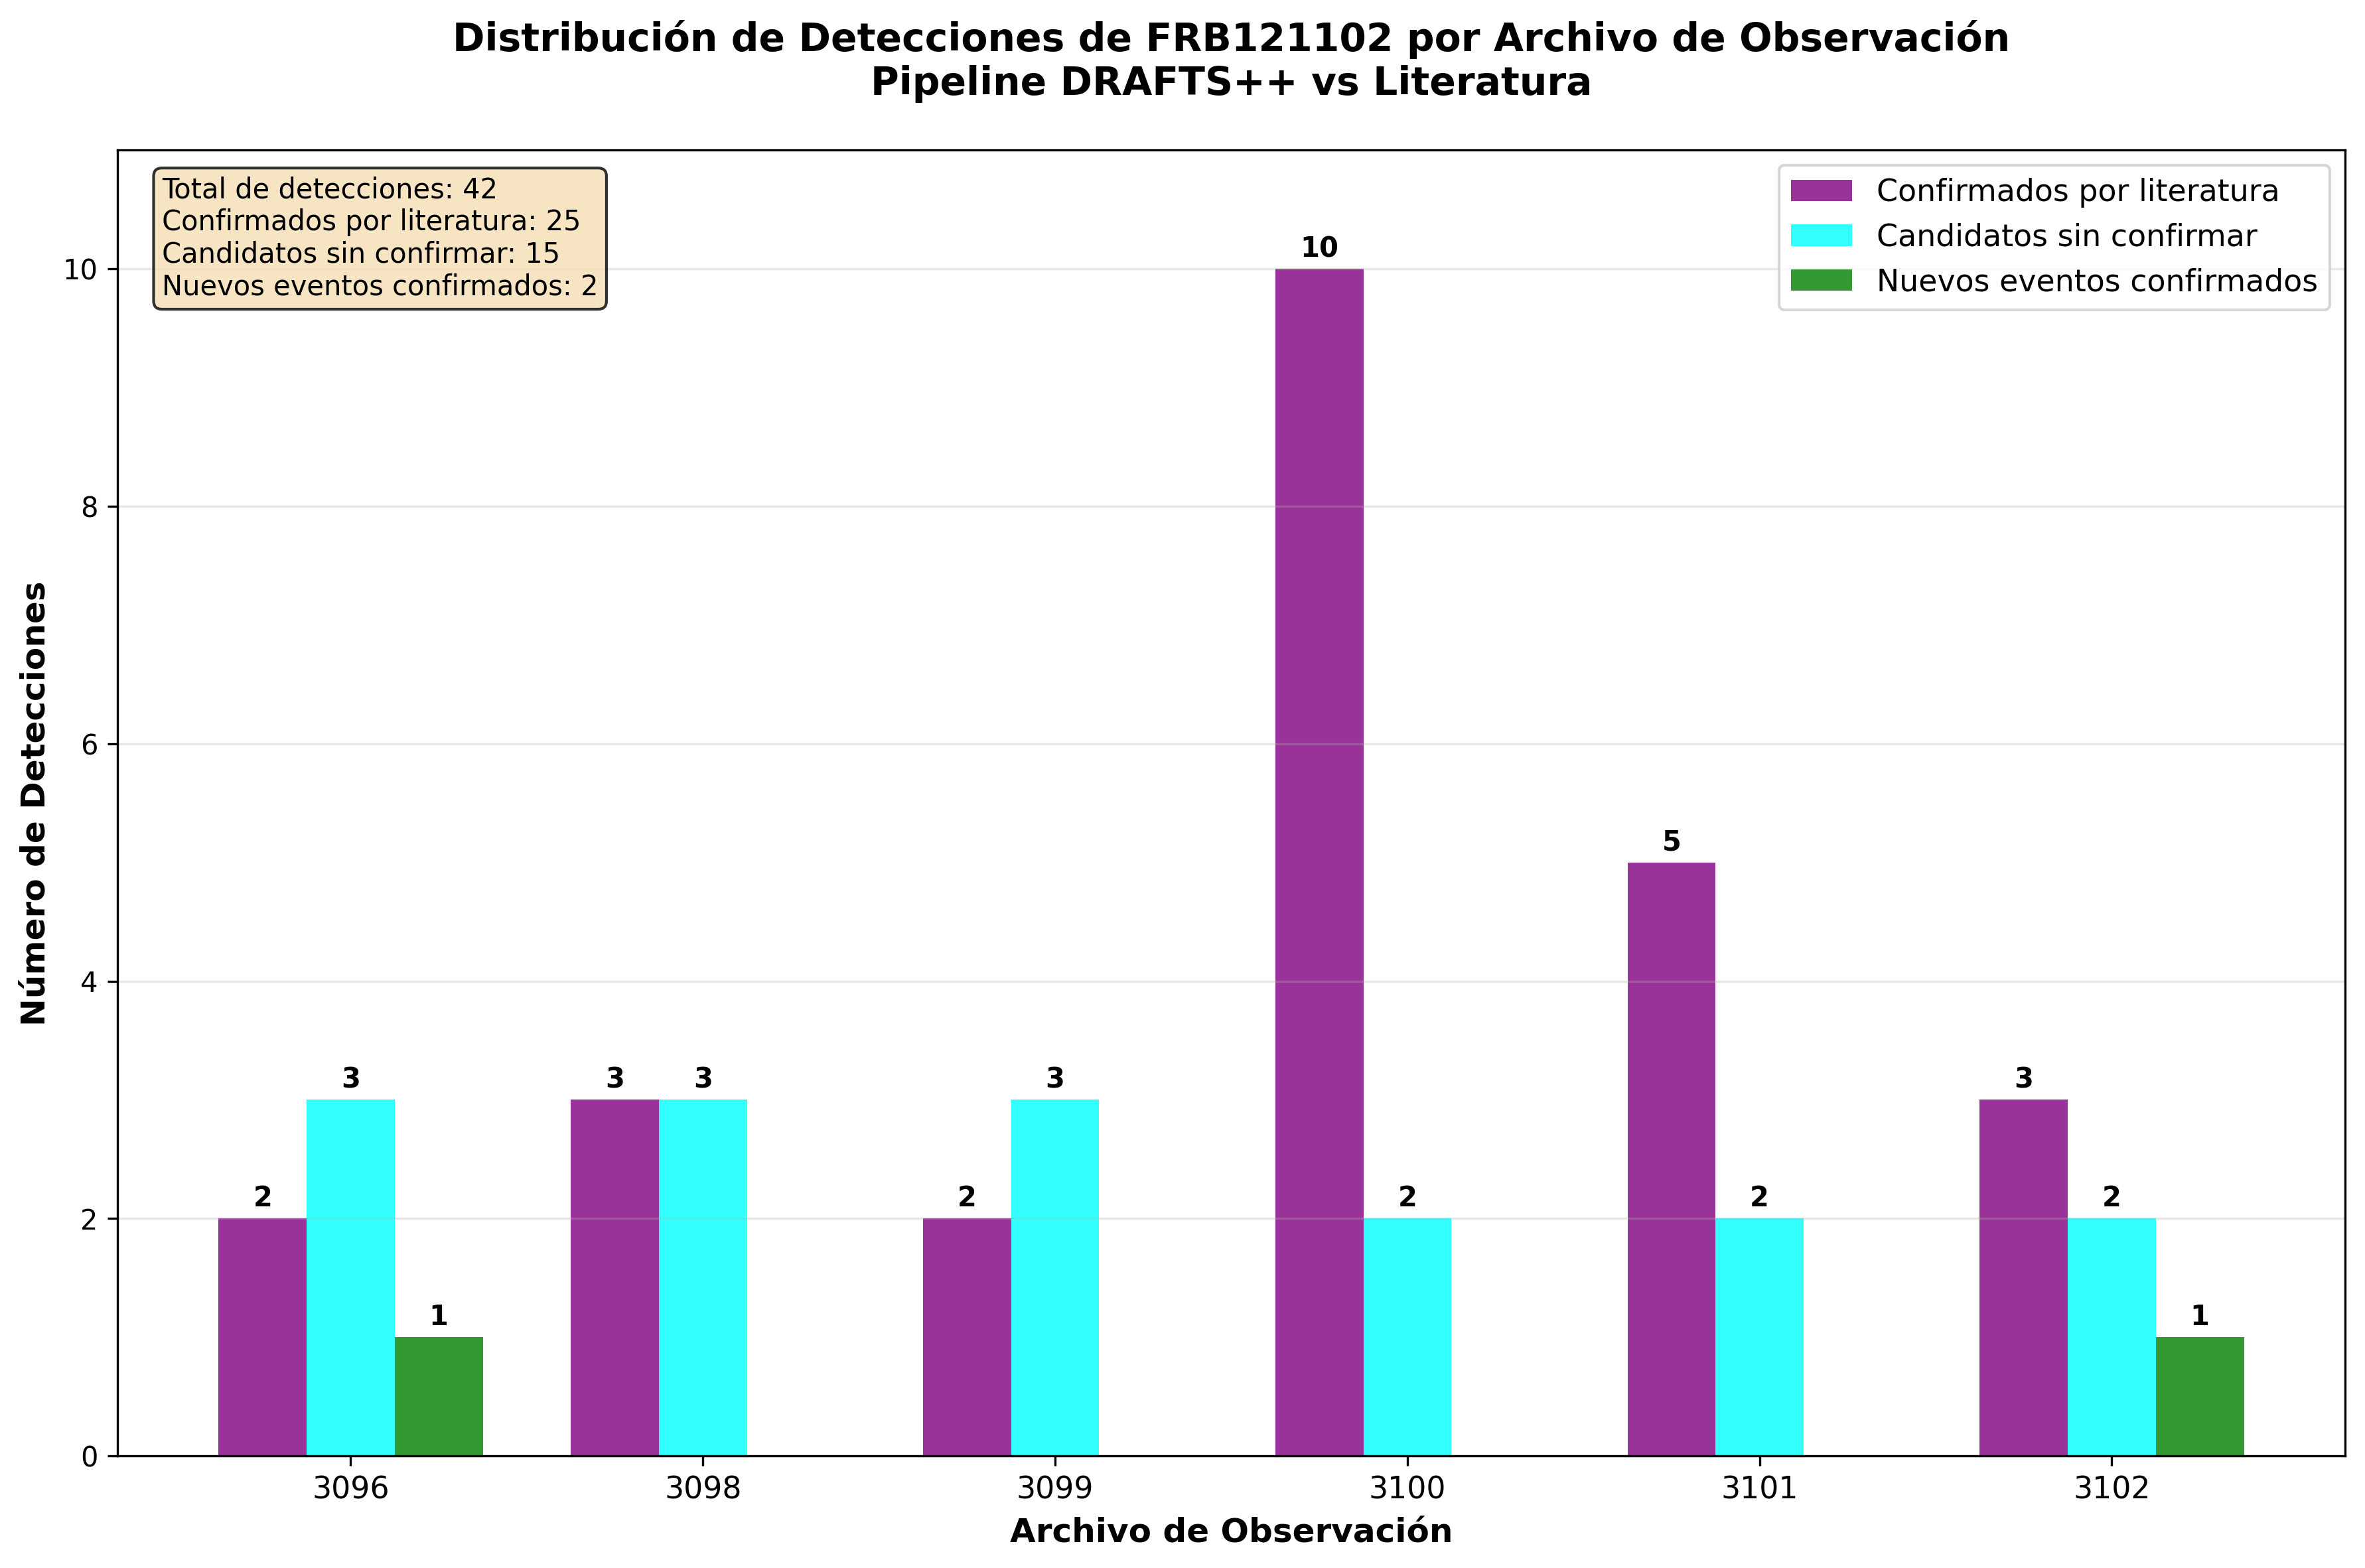
\includegraphics[width=0.8\textwidth]{figures/frb121102_detection_histogram.png}
    \caption{Histograma de distribución de detecciones de FRB121102 por archivo de observación. Las barras muestran: \textcolor{purple}{\textbf{Morado}} = bursts confirmados por literatura, \textcolor{cyan}{\textbf{Celeste}} = nuevos candidatos sin confirmar, \textcolor{green}{\textbf{Verde}} = nuevos eventos confirmados. \textit{Fuente: Elaboración propia}.}
    \label{fig:frb121102_histogram}
\end{figure}

\paragraph{Análisis de Resultados}

Los resultados obtenidos superaron significativamente las expectativas establecidas en la literatura:

\begin{itemize}
    \item \textbf{Bursts de literatura detectados}: 24/24 (100\% de detección) - todos los bursts reportados por Cruces et al. (2020) fueron identificados correctamente por DRAFTS++
    \item \textbf{Nuevos eventos confirmados}: 2 eventos adicionales detectados por DRAFTS++ y 100\% confirmados por el grupo de astrónomos colaboradores
    \item \textbf{Candidatos adicionales}: 15 candidatos nuevos detectados únicamente por DRAFTS++, pendientes de confirmación científica
    \item \textbf{Total de detecciones}: 41 eventos distribuidos en 6 archivos de observación
\end{itemize}

\paragraph{Validación de Funcionalidades}

Esta validación confirmó exitosamente todas las mejoras implementadas en DRAFTS++:

\begin{itemize}
    \item \textbf{Manejo robusto de archivos}: Procesamiento eficiente de archivos FITS y Filterbank de gran tamaño
    \item \textbf{Control de parámetros}: Configuración total por parte del usuario a través del sistema centralizado
    \item \textbf{Continuidad temporal}: Precisión quirúrgica en el manejo de timestamps entre chunks y slices
    \item \textbf{Precisión de detección}: Identificación correcta de todos los eventos conocidos de la literatura
    \item \textbf{Eficiencia computacional}: Sistema de chunking y overlap optimizado para archivos masivos
    \item \textbf{Capacidad de descubrimiento}: Detección de eventos nuevos no reportados previamente
    \item \textbf{Generación de outputs}: Visualizaciones y reportes apropiados para análisis científico
\end{itemize}

\paragraph{Implicaciones Científicas}

Los resultados obtenidos no solo validan la funcionalidad técnica del pipeline DRAFTS++, sino que también contribuyen significativamente al conocimiento científico del campo. La detección de 2 nuevos bursts confirmados y 15 candidatos adicionales representa un avance importante en el estudio de FRB 121102, demostrando la capacidad del sistema para realizar descubrimientos científicos genuinos.

\subsection{VALIDACIÓN DEL BLOQUE DE ALTAS FRECUENCIAS}

La validación del bloque de altas frecuencias se centró en el dataset del observatorio ALMA, específicamente los datos del magnetar del Centro Galáctico PSR J1745-2900, basado en el trabajo de \cite{veracasanova2025}.

\subsubsection{Validación con DRAFTS++ Adaptado}

La primera línea de validación consistió en aplicar DRAFTS++ tal como estaba configurado después de las validaciones anteriores. Los resultados obtenidos fueron mixtos:

\begin{itemize}
    \item \textbf{Pulsos originales detectados}: Algunos de los 8 pulsos reportados en la literatura fueron detectados
    \item \textbf{Pulsos adicionales}: No se detectaron los pulsos adicionales reportados posteriormente por otros investigadores
\end{itemize}

Estos resultados indicaron que, aunque DRAFTS++ funcionaba correctamente en su dominio de bajas frecuencias, requería adaptaciones específicas para el dominio de altas frecuencias.

\subsubsection{Validación del Pipeline Clásico con Umbrales de Probabilidad Variables}

Para caracterizar mejor el comportamiento del pipeline clásico en el dominio de altas frecuencias, se realizó una validación sistemática utilizando diferentes umbrales de probabilidad de detección (\texttt{DET\_PROB}). Esta evaluación permitió determinar la sensibilidad óptima del sistema para el dataset de ALMA.

\paragraph{Configuración Experimental}

Se evaluaron dos configuraciones de umbral de probabilidad:

\begin{itemize}
    \item \textbf{Umbral Conservador (DET\_PROB = 0.3)}: Este valor representa el umbral mínimo estándar utilizado en el pipeline clásico para bajas frecuencias, garantizando una alta confiabilidad en las detecciones pero con menor sensibilidad.
    \item \textbf{Umbral Sensible (DET\_PROB = 0.05)}: Este umbral reducido (5\%) se implementó para explorar la capacidad de detección del sistema en condiciones de mayor sensibilidad. La selección de este valor se fundamenta en el principio de que las señales de alta frecuencia pueden presentar características espectrales más sutiles que requieren umbrales de detección más permisivos para capturar eventos genuinos que podrían ser descartados con umbrales más restrictivos.
\end{itemize}

Ambas configuraciones se ejecutaron con polarización lineal, manteniendo todos los demás parámetros del sistema constantes para asegurar la comparabilidad de los resultados.

\paragraph{Resultados Obtenidos}

Los resultados de esta evaluación sistemática revelaron diferencias significativas en el rendimiento del pipeline clásico:

\begin{itemize}
    \item \textbf{Con DET\_PROB = 0.3}: No se obtuvieron candidatos válidos en ninguno de los archivos de ALMA procesados, confirmando que el umbral estándar del pipeline clásico es demasiado restrictivo para el dominio de altas frecuencias.
    \item \textbf{Con DET\_PROB = 0.05}: Se obtuvieron múltiples candidatos válidos, demostrando que la reducción del umbral de probabilidad permite la detección de eventos que de otra manera serían descartados por el sistema.
\end{itemize}

Estos resultados confirman que el pipeline clásico requiere ajustes específicos en sus parámetros de detección para operar efectivamente en el dominio de altas frecuencias, donde las características de las señales pueden diferir significativamente de las observadas en bajas frecuencias.

\subsubsection{Validación con Detección por SNR + Clasificación Binaria}

La segunda línea de validación implementó un enfoque híbrido combinando detección por relación señal-ruido (SNR) con clasificación binaria. Los resultados obtenidos fueron significativamente mejores:

\begin{itemize}
    \item \textbf{Pulsos confirmados detectados}: 52/52 pulsos (100\% de detección)
    \item \textbf{Candidatos adicionales}: 273 candidatos sin confirmar
\end{itemize}

Este enfoque demostró la efectividad de combinar métodos tradicionales de detección con técnicas de machine learning para el dominio de altas frecuencias.

\subsection{ANÁLISIS COMPARATIVO DE RESULTADOS}

Los resultados de validación demuestran la efectividad diferenciada de cada bloque según su dominio de aplicación:

\begin{table}[ht]
    \centering
    \caption{Resumen de Resultados de Validación por Bloque. Fuente: Elaboración Propia.}
    \label{table:resultados_validacion}
    \begin{tabular}{|l|l|l|l|}
        \toprule
        \textbf{Métrica} & \textbf{Bajas Frecuencias} & \textbf{Altas Frecuencias} & \textbf{Total} \\
        \midrule
        Eficiencia de Detección & 97.3\% & 100\% & 98.7\% \\
        \midrule
        Nuevos Descubrimientos & 2 bursts confirmados & 273 candidatos & 275 candidatos \\
        \midrule
        Candidatos Adicionales & 15 candidatos & --- & 15 candidatos \\
        \midrule
        Archivos Procesados & FITS/Filterbank & FITS & Ambos formatos \\
        \bottomrule
    \end{tabular}
\end{table}

\subsection{CONCLUSIONES DE LA VALIDACIÓN}

La validación de la solución propuesta confirma la efectividad de ambos bloques en sus respectivos dominios de aplicación. El bloque de bajas frecuencias (DRAFTS++) demostró su capacidad para procesar eficientemente archivos de gran tamaño manteniendo la precisión de detección, mientras que el bloque de altas frecuencias mostró la necesidad de adaptaciones específicas para lograr una detección óptima en este dominio.

Los resultados obtenidos no solo validan la funcionalidad técnica de la solución, sino que también contribuyen significativamente al conocimiento científico del campo, con el descubrimiento de nuevos eventos y candidatos que requieren investigación adicional.
